\chapter{Experiment}
We conducted two sets of experiments to evaluate the system's localization accuracy: one on point localization and the other on movement tracking. 

\section{Setup}
\subsection{Point localization}

\begin{figure}[]
  \centering
  \begin{subfigure}[]{.48\textwidth}
    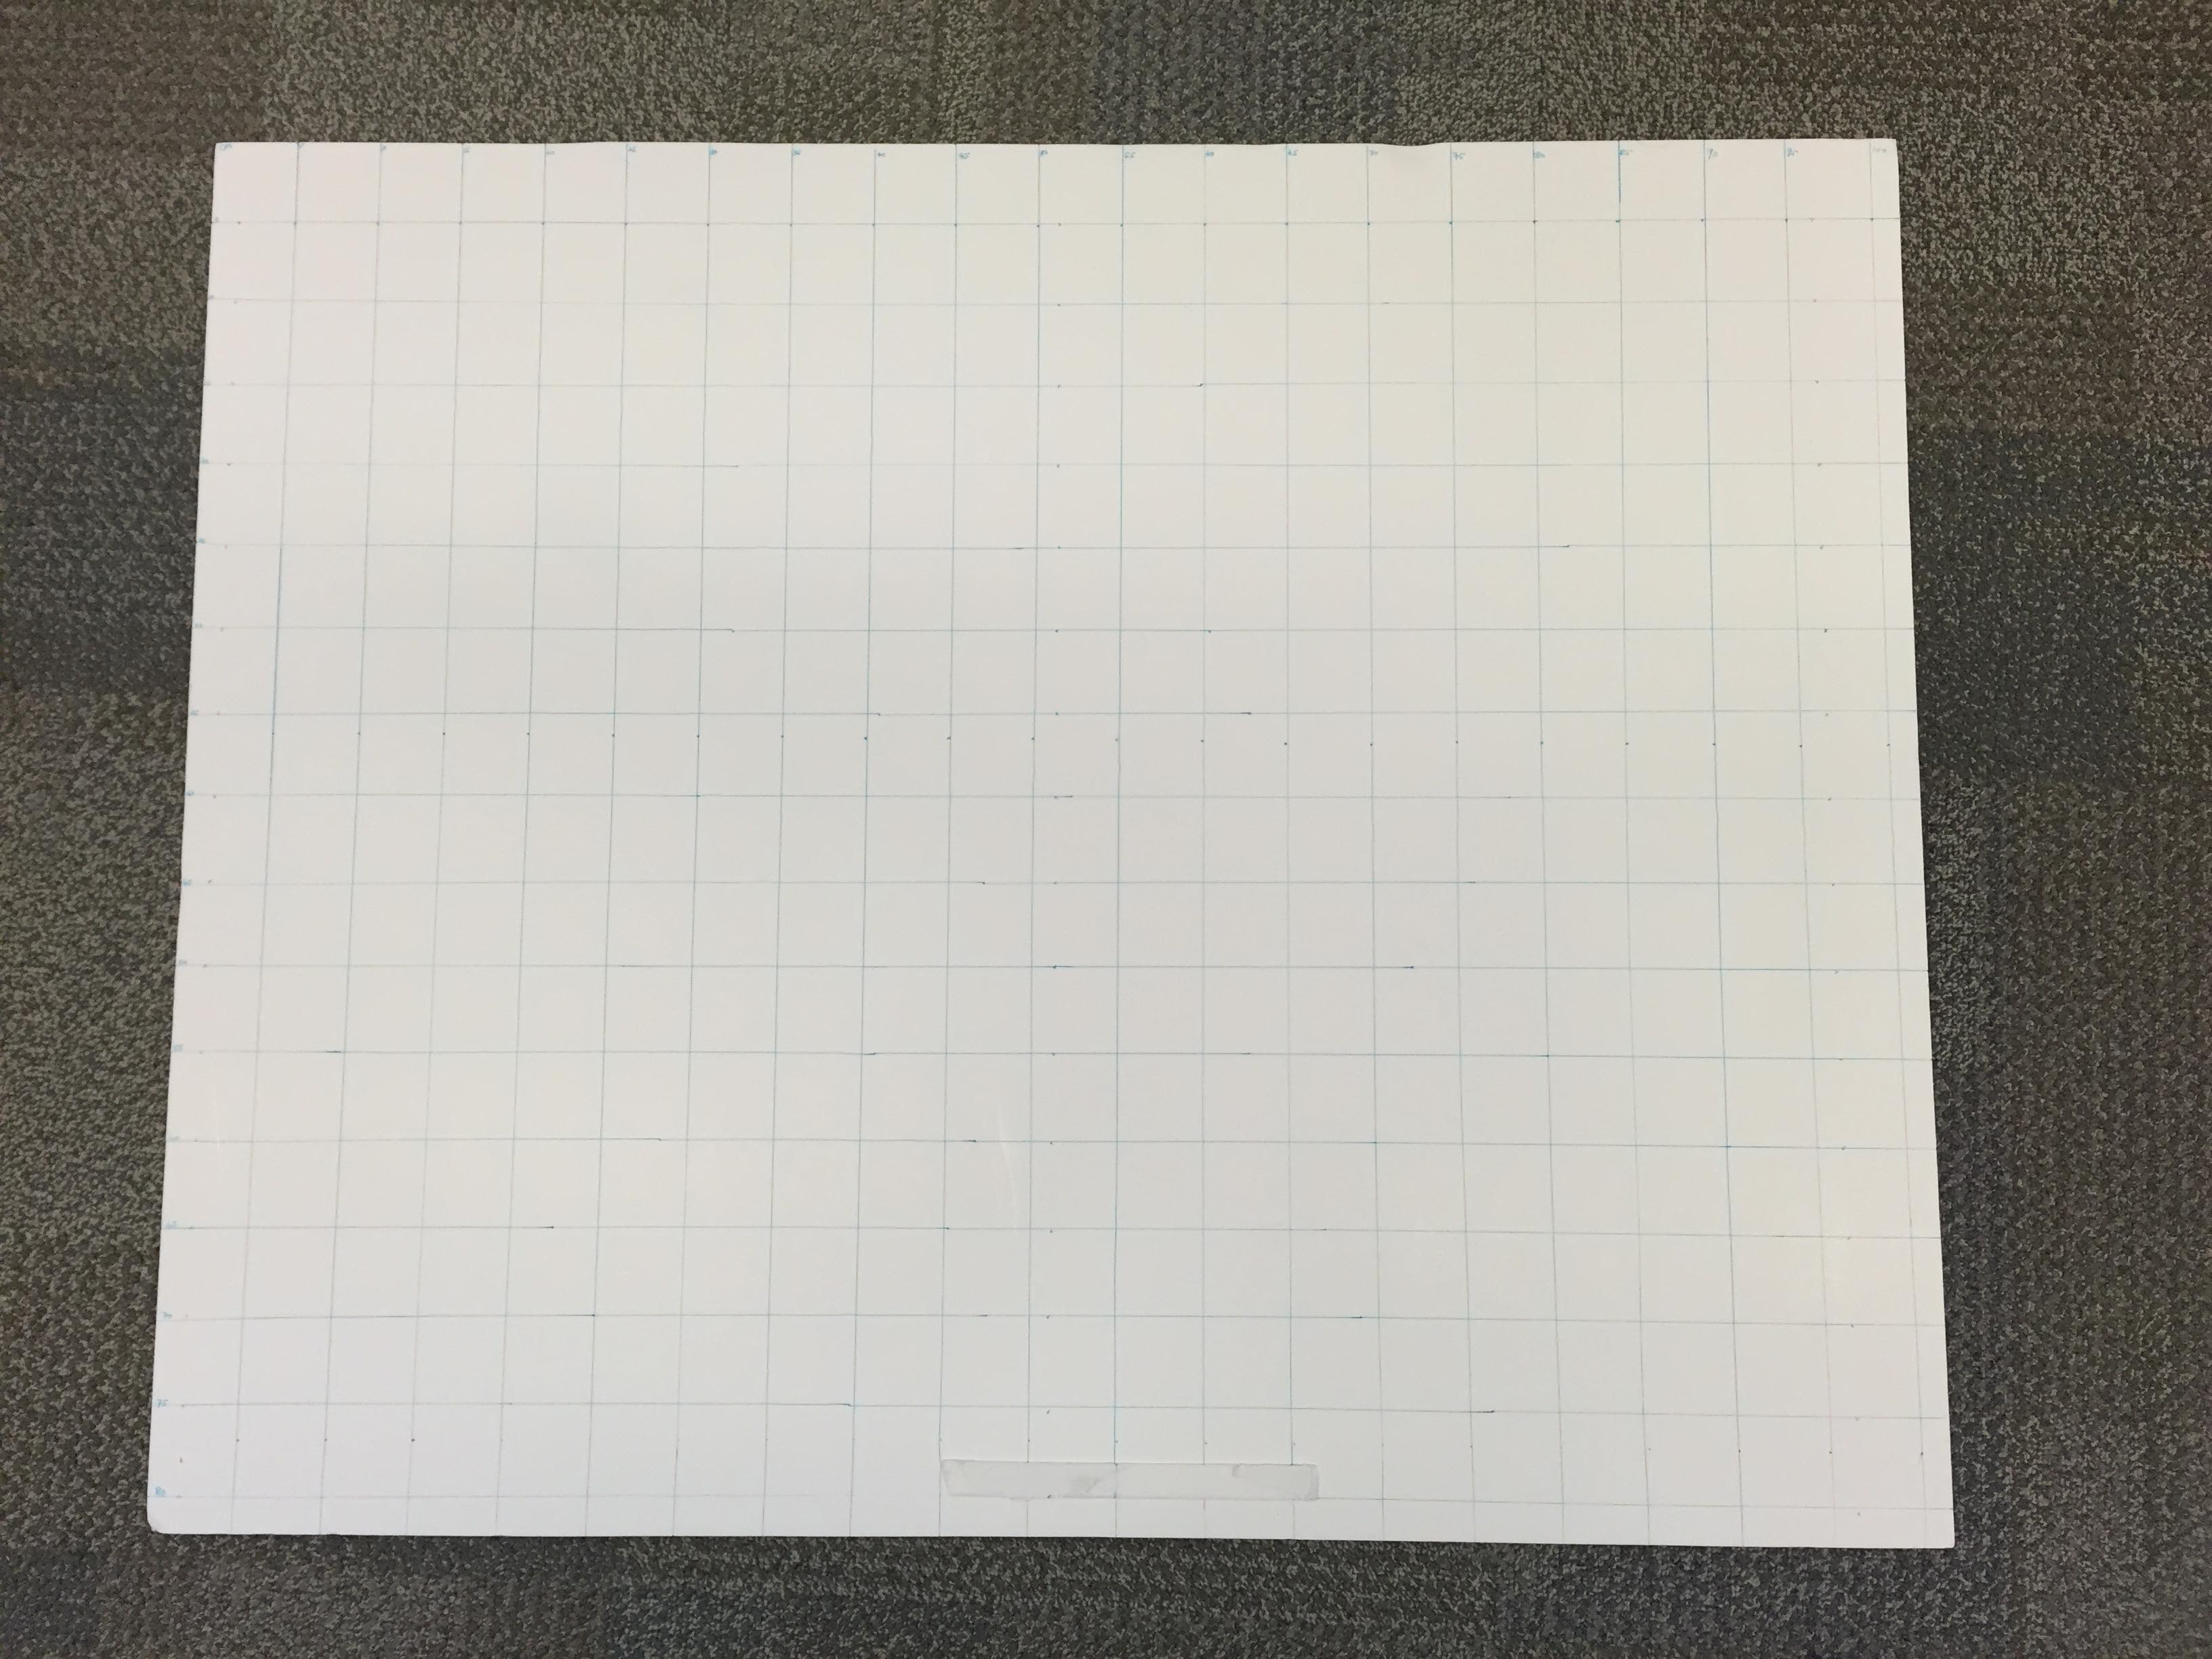
\includegraphics[width=\textwidth]{setup_1.JPG}
    \caption{1 meter by 1 meter grid}
  \end{subfigure}
  \begin{subfigure}[]{.48\textwidth}
    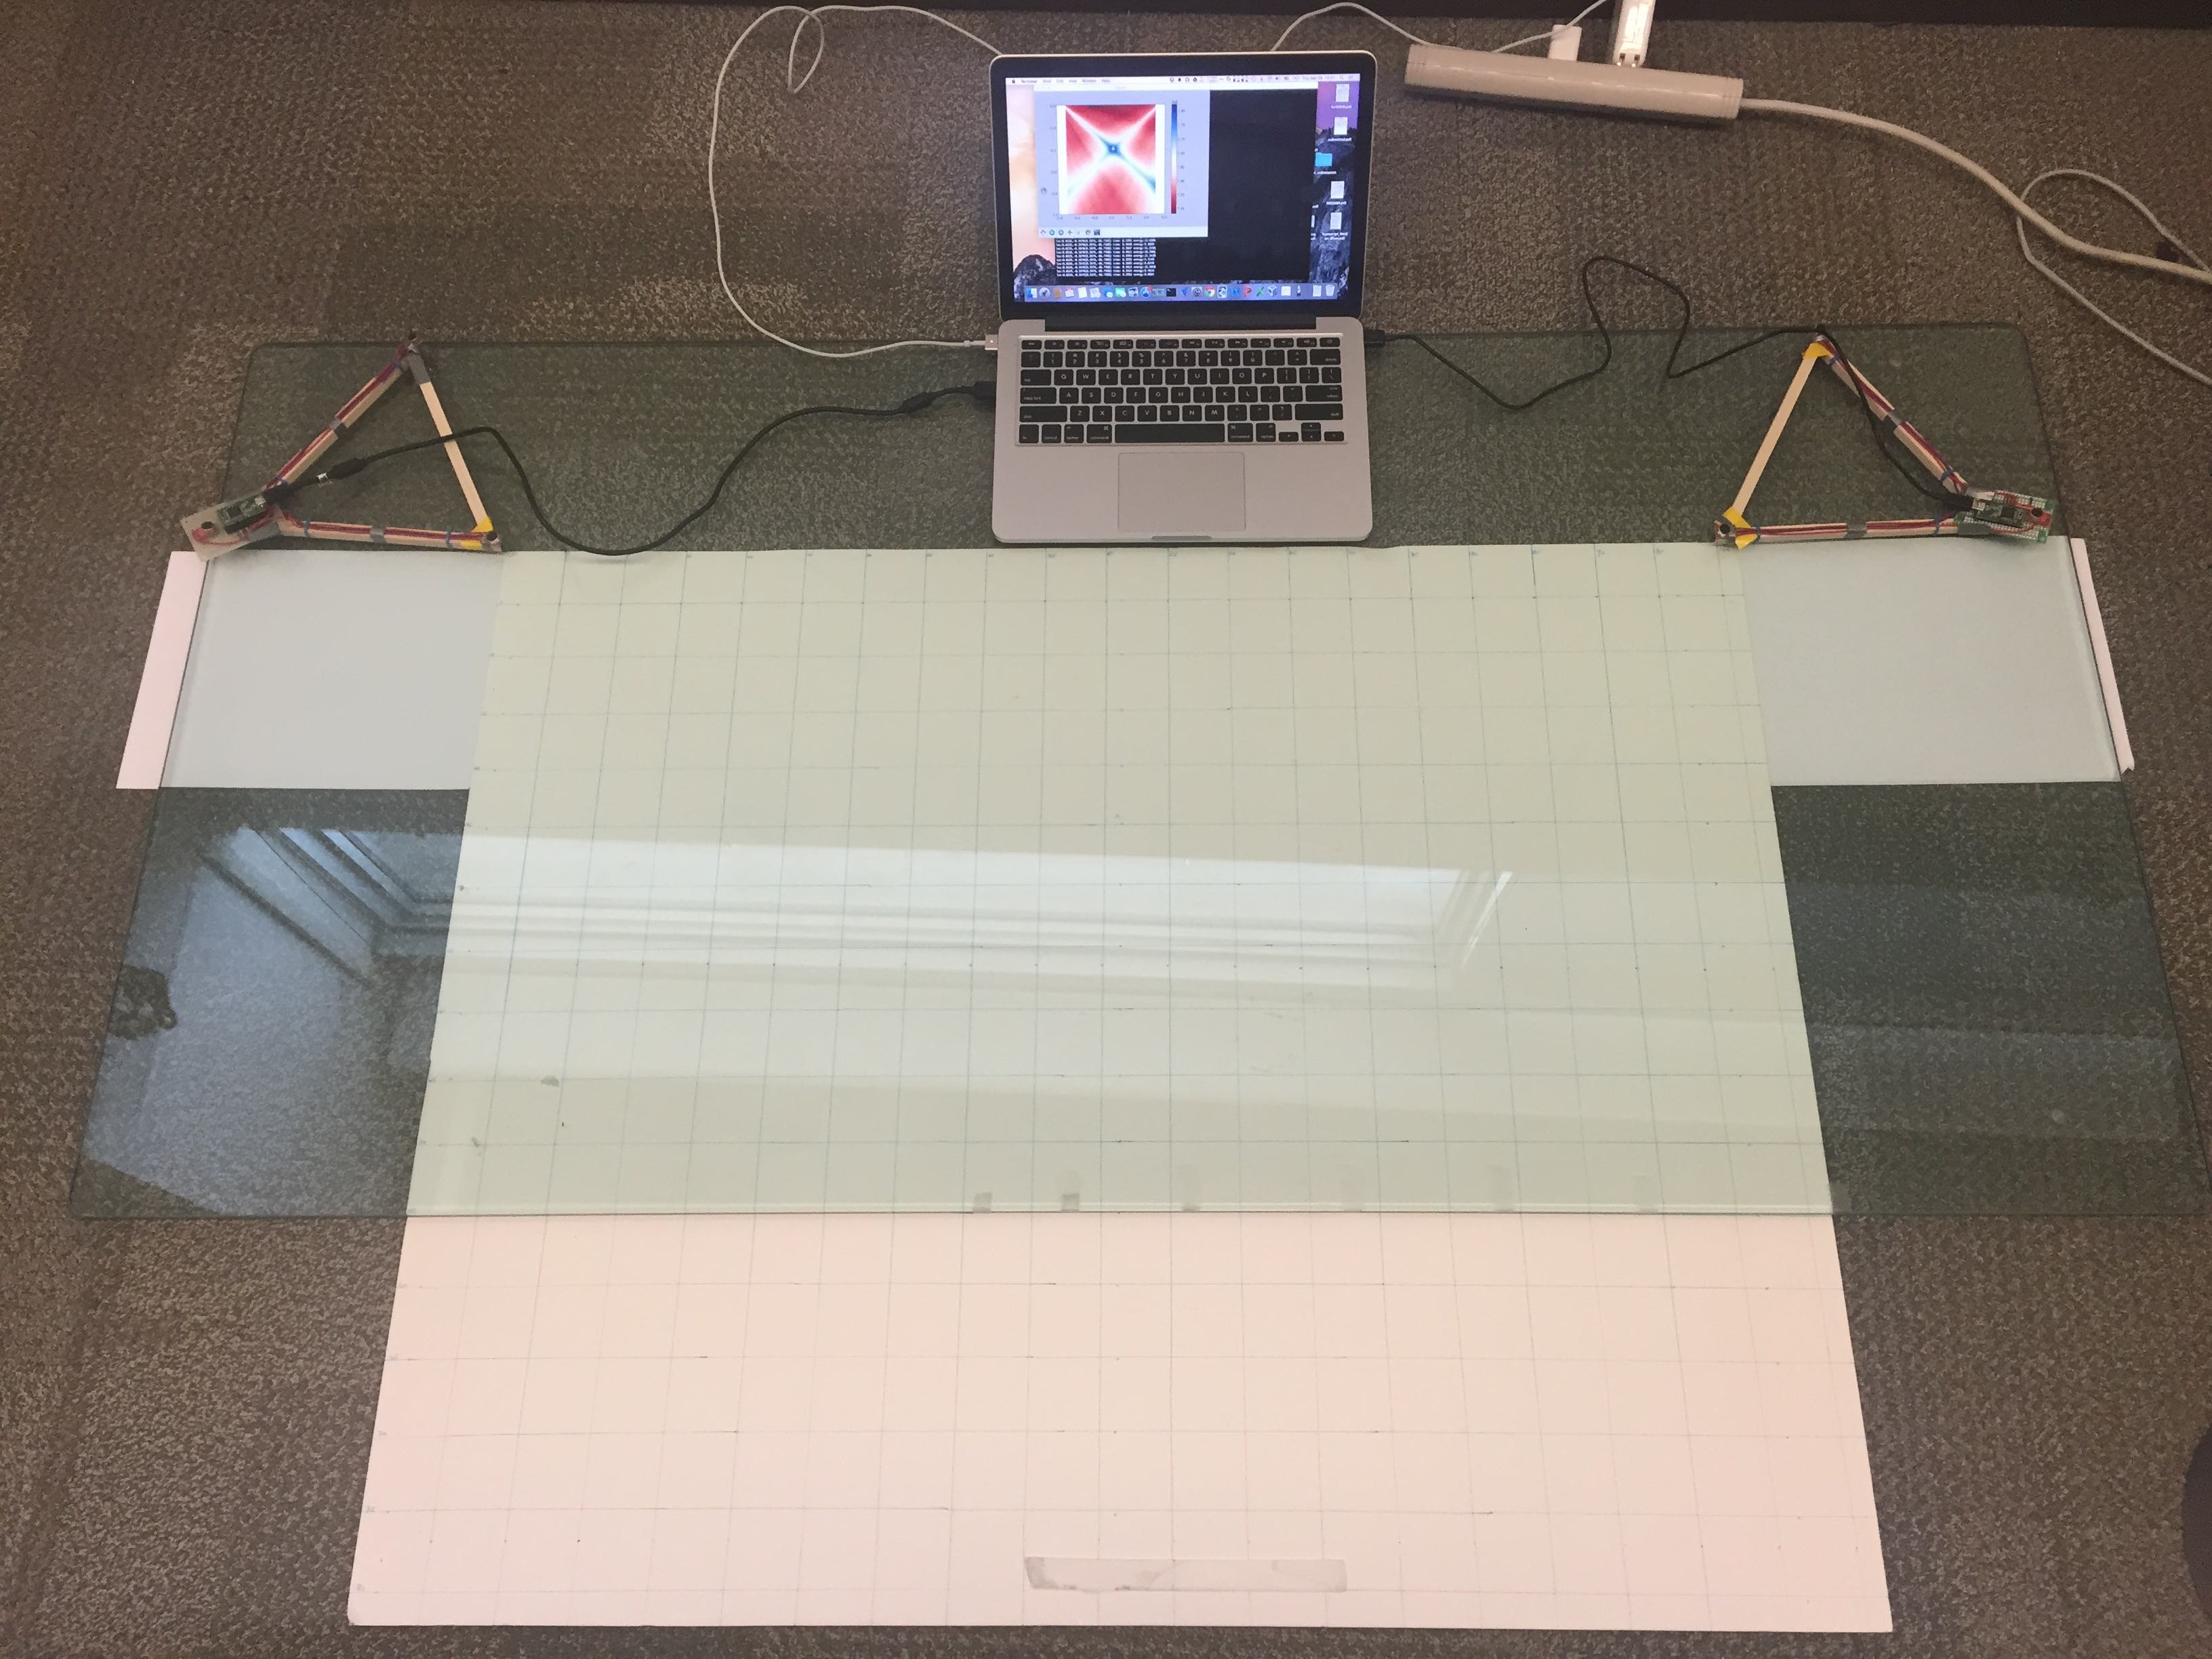
\includegraphics[width=\textwidth]{setup_2.JPG}
    \caption{array placement}
  \end{subfigure}
  \caption{Setup for point localization evaluation}
  \label{fig:setup_point}
\end{figure}

An one meter by one meter grid was set up where the arrays were placed at the top left and top right corners of the grid. Fig~\ref{fig:setup_point} shows a picture of the setup. A total of $32$ testing locations were chosen uniformly in this grid. We reported the error as the average distance between our placement of the audio source and the location estimated from the arrays.

\subsection{Movement tracking}
To test how well the system tracks movement, we mounted a rotating disk $40$ centimeters in diameter onto the grid at $(x=0$ cm$, y=-30$ cm$)$. Fig~\ref{fig:setup_circle} shows a picture of the setup. A sound source is placed on the edge of the rotating disk and the arrays track the sound source as it rotates in a circle. In this experiment, we evaluated how accuracy changes with:
\begin{itemize}
\item window sizes
\item audio sources
\item movement tracking filters
\item movement speeds
\end{itemize}

To test how different sound sources impact localization quality, we conducted the experiments with three different sound sources:
\begin{description}%[\IEEEsetlabelwidth{long a label}\IEEEusemathlabelsep]

\item[White Noise] A recording of white noise.

\item[Music A] A randomly picked music that has normal audio amplitude throughout the experiment period. \emph{Honest Eyes} by \emph{Black Tide} was the music used.

\item[Music B] A randomly picked music with intermittent low amplitude sections. \emph{Canon} was the music used.

\end{description} 

To test how the movement speed of sound source affects localization quality, each experiment was conducted at two different speeds:
\begin{description}
\item[Normal] An angular speed of $0.5$ rad/s was maintained, which translates to a linear speed of $10$ cm/s.
\item[Fast] An angular speed of $1.0$ rad/s was maintained, which translates to a linear speed of $20$ cm/s.
\end{description}

For each experiment conducted, two different movement filters were evaluated:
\begin{description}%[\IEEEsetlabelwidth{Very long label}\IEEEusemathlabelsep]
\item[Averaging filter] localization for past $0.5$ seconds were averaged and outputted as current estimate.
\item[Kalman filter] A 2nd order Kalman filter was used.
\end{description}

In the movement tracking experiments described above, we have the ground truth location of the circle, but not the exact location of the audio source at each moment during the movement. Therefore, the error is reported as the distance between the localized point to its closest point on the ground truth circle.

\section{Results}
\subsection{Point localization}
To test how accuracy varies with window size, the algorithm is fed with microphone data of different lengths, and the result is shown in fig~\ref{fig:accuracy_vs_window}. The error decreases as window size increases and plateaus after the window size exceeds around $10$ millisecond. The lowest error achieved is $2.53$ centimeters, which occurred when the window size is set to 12 millisecond and GCC\_PHAT is used for TDOA estimation.

Although accuracy improves with the window size, computation time also increases with it. The part of calculation that depends on the window size is using cross correlation for TDOA estimation. Cross correlation can be calculated with Fast Fourier Transform (FFT) and the runtime is of order $O(N\log N)$. We measured how the computation time varied with window size and Figure~\ref{fig:speed_vs_window} shows the result. The runtime increases approximately linearly in the window size region of interest.

We also calculated the localization error for each tested point in the grid. Figure~\ref{fig:error_distribution} shows the error distribution inside the grid. The error is below $3$ cm for most areas inside the grid. There is one error spike in the mid-left region and we contribute this to audio source misplacement because the error is fairly low and consistent around that spike.

To test the limit of the system and to evaluate the accuracy when the source moves outside of the one meter by one meter region, we measured the localization error by placing the source at $10$ locations along $y$ axis ranging from $(0$ cm$, -10$ cm$)$ to $(0$ cm$, -200$ cm$)$. The result is presented in fig~\ref{fig:error_along_y}. The localization error is within $3$ cm when the source is within $100$ cm from the arrays. The error increases to about $5$ cm when the source distance increases to $150$ cm and the error exceeds $10$ cm after the source distance reaches $200$ cm.

\begin{figure}[]
\centering
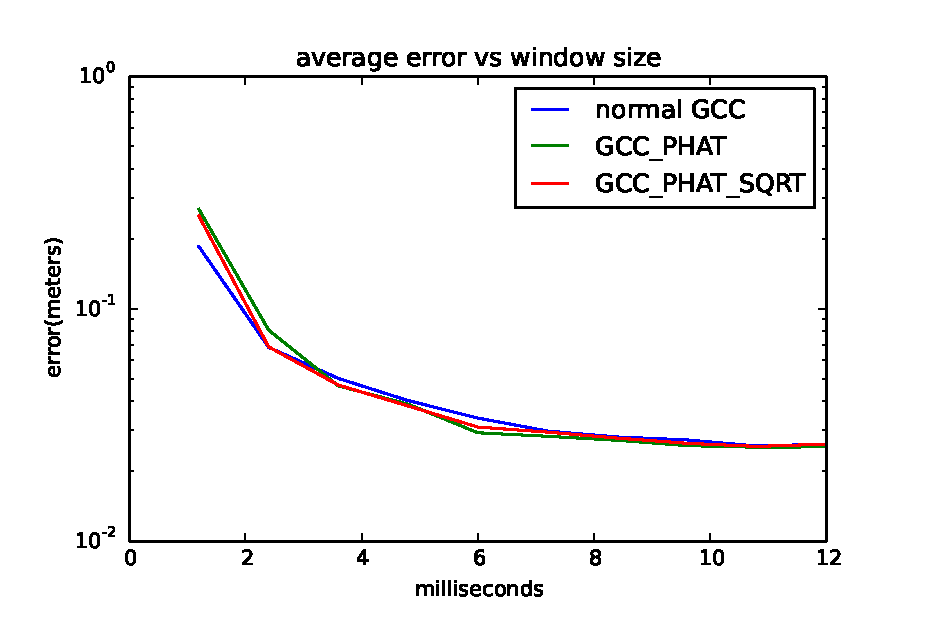
\includegraphics[width=1.0\textwidth]{average_error_window_size.eps}
\caption{Localization error versus window size}
\label{fig:accuracy_vs_window}
\end{figure}

\begin{figure}[]
\centering
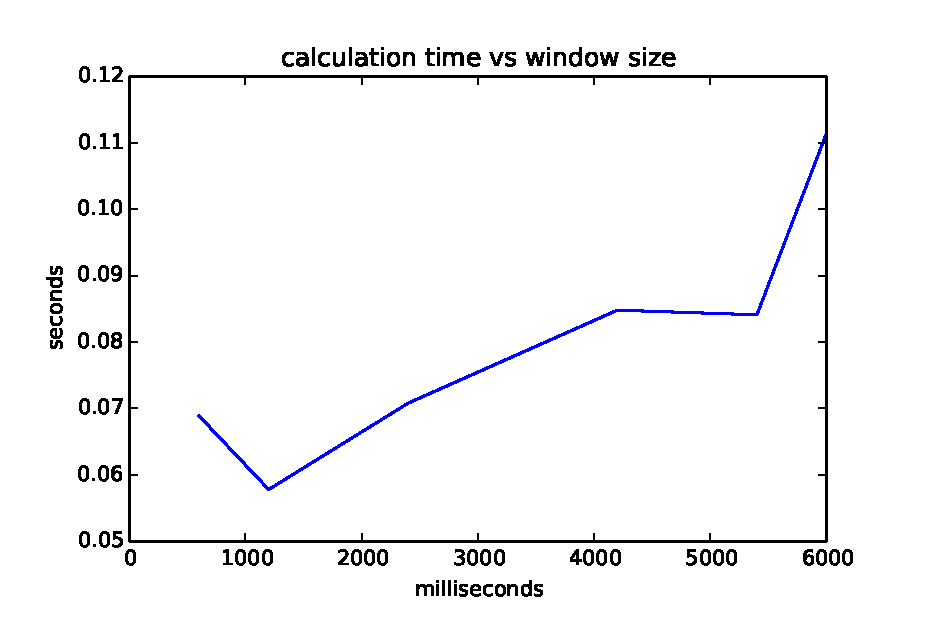
\includegraphics[width=1.0\textwidth]{calculation_time.eps}
\caption{Computation time versus window size}
\label{fig:speed_vs_window}
\end{figure}


\begin{figure}[]
\centering
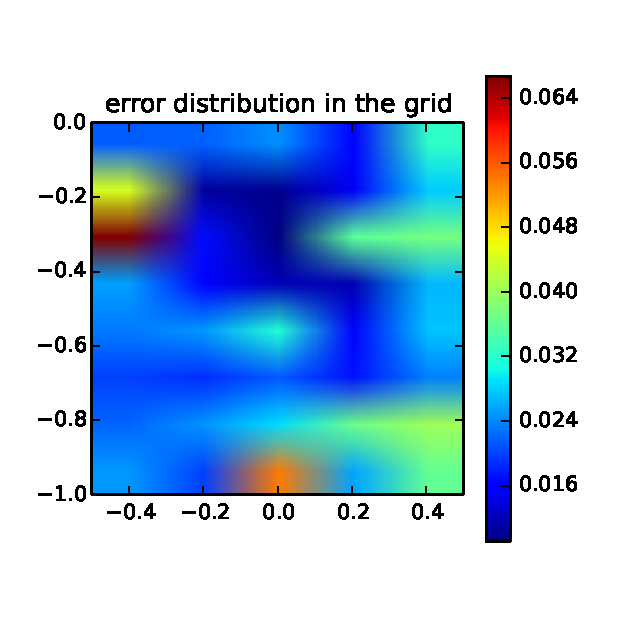
\includegraphics[width=1.0\textwidth]{error_distribution.eps}
\caption{error distribution in the grid. Arrays are placed at $(-0.5$ m$, 0$ m$)$ and $(0.5$ m$, 0$ m$)$}
\label{fig:error_distribution}
\end{figure}

\begin{figure}[]
\centering
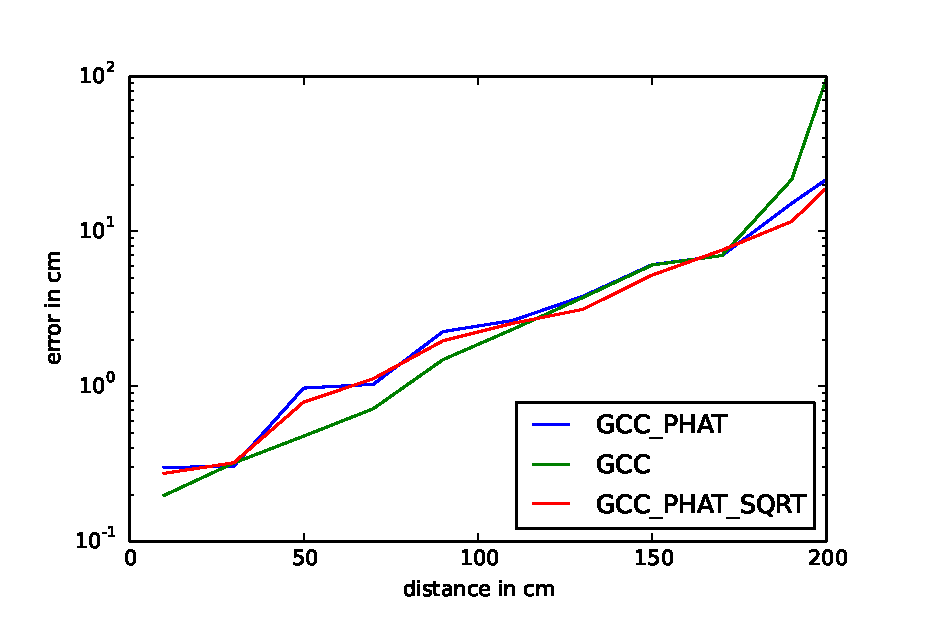
\includegraphics[width=1.0\textwidth]{error_along_y_axis.eps}
\caption{Localization error as the distance between the source and the microphone arrays increases. The source is placed on the $y$ axis.}
\label{fig:error_along_y}
\end{figure}


\begin{figure}[]
  \centering
%  \begin{subfigure}[]{.2\textwidth}
%    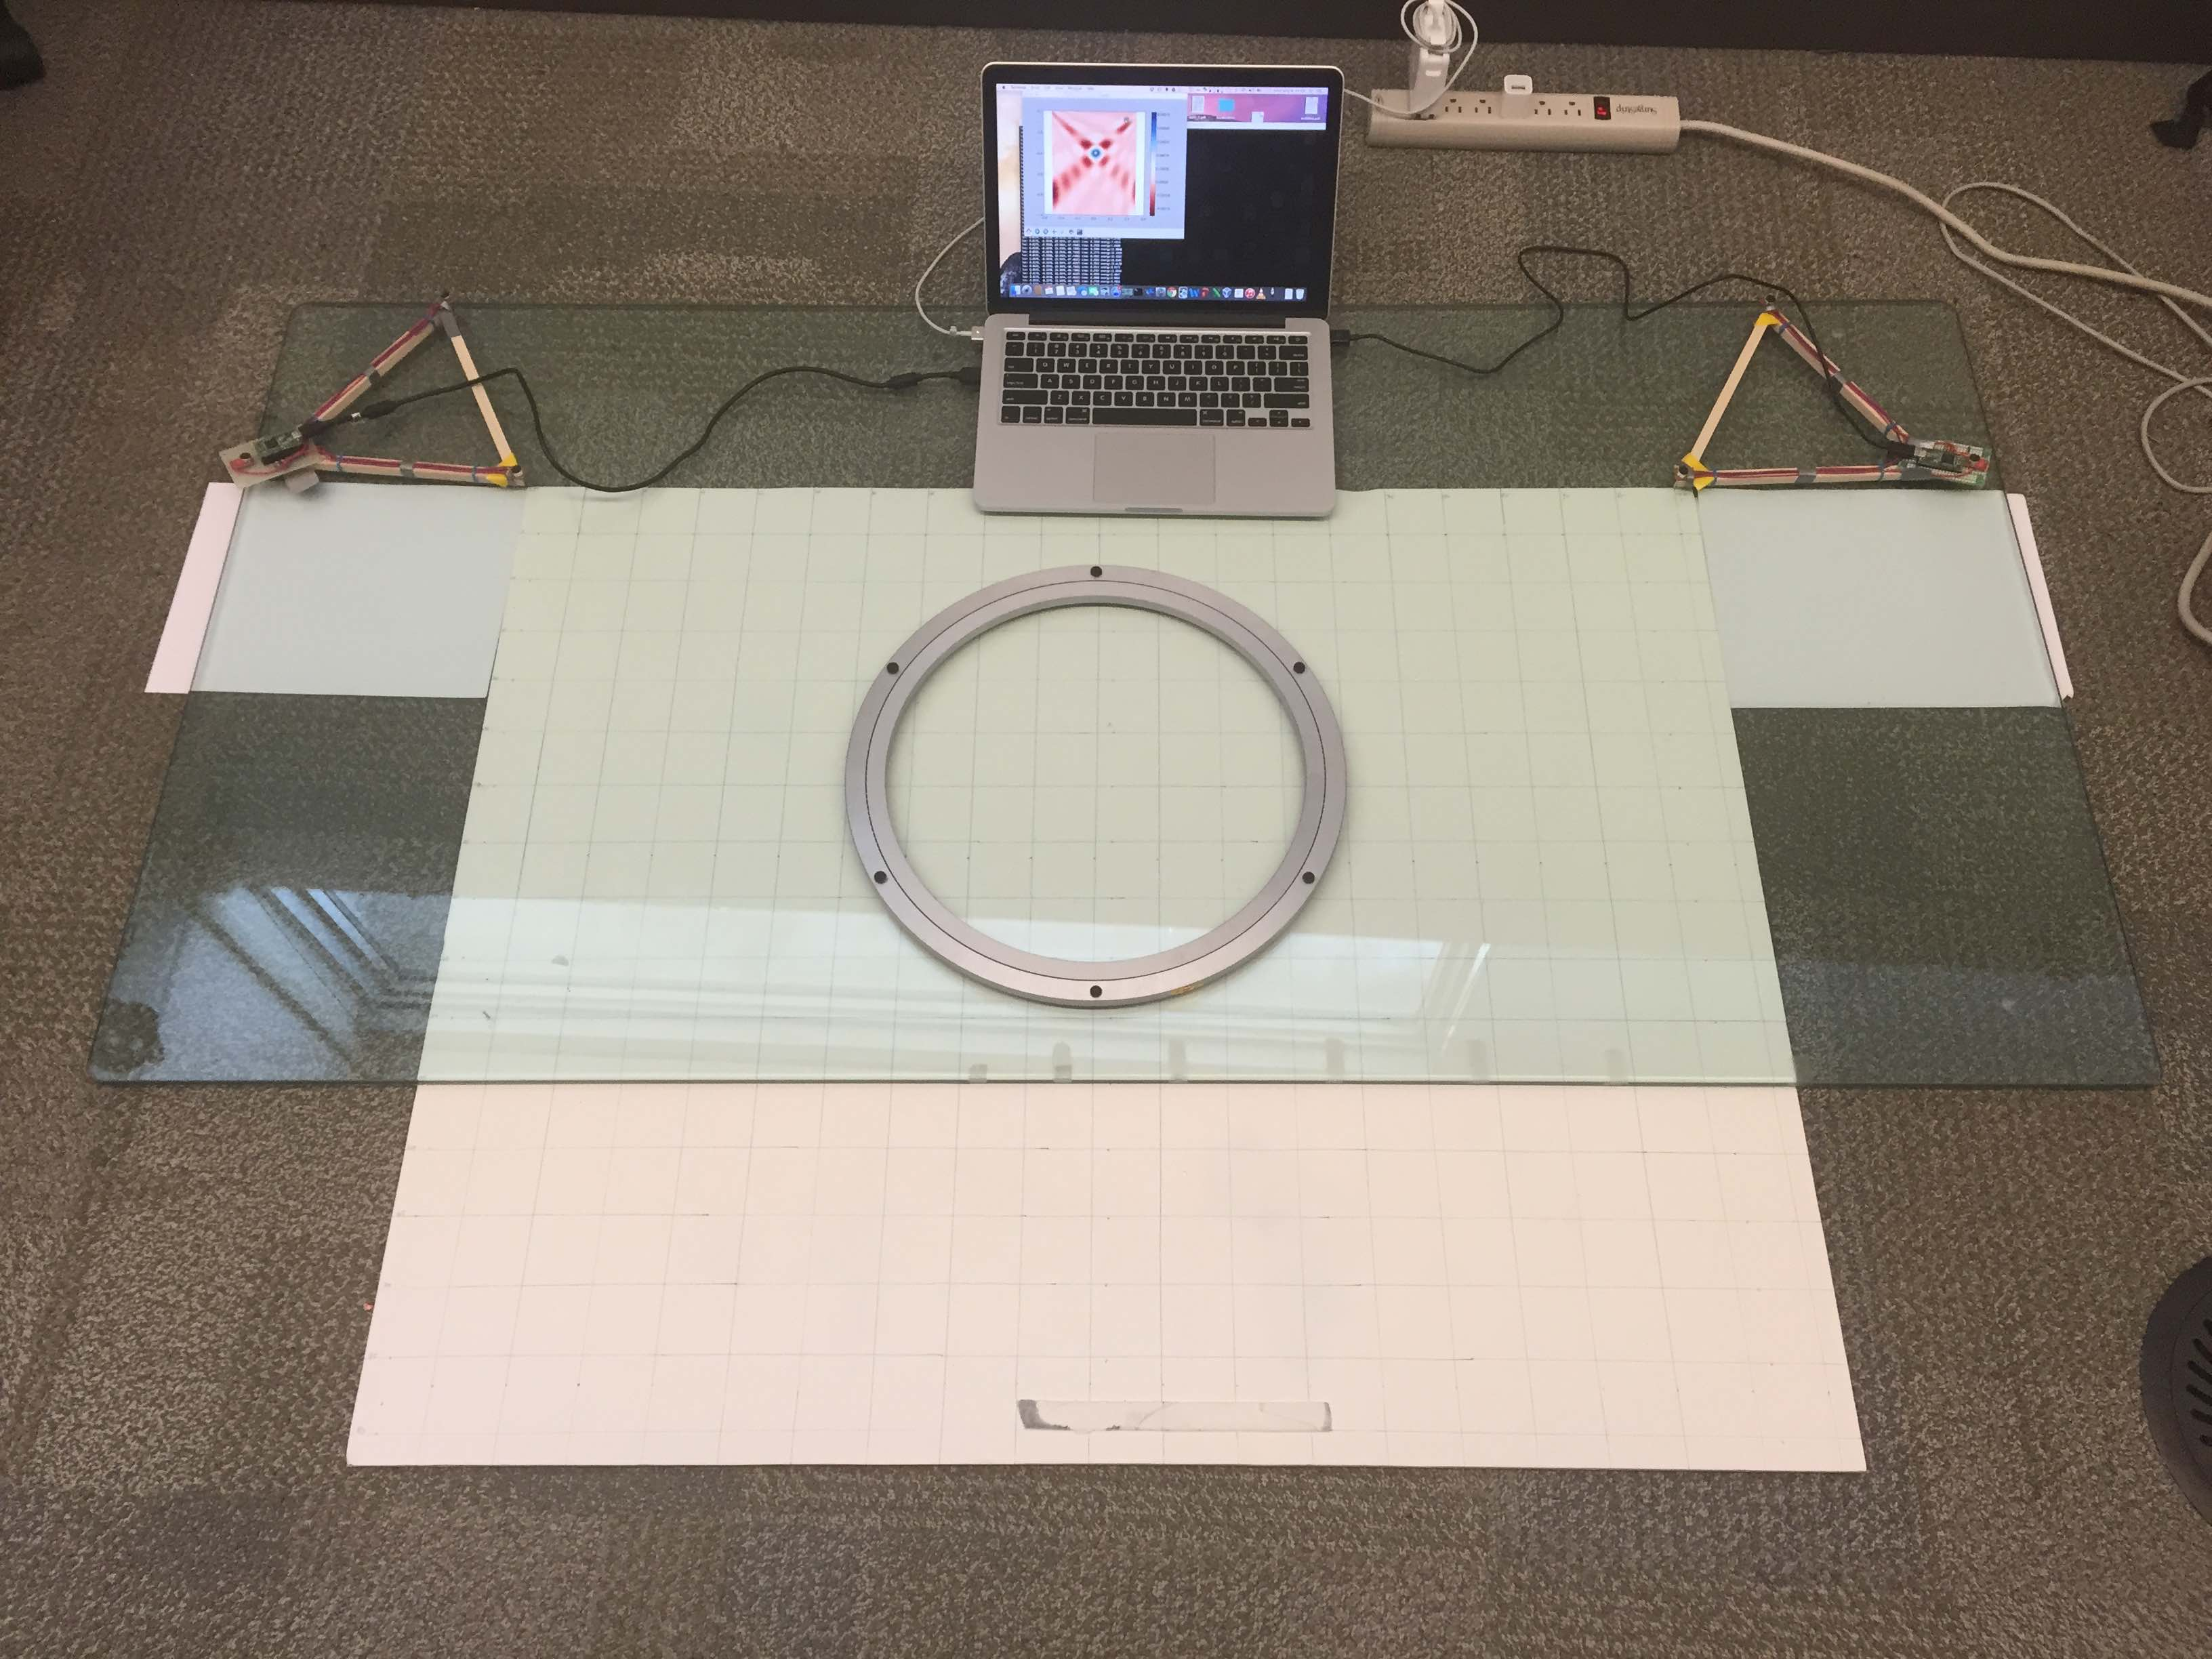
\includegraphics[width=\textwidth]{setup_ring.JPG}
%  \end{subfigure}
  \begin{subfigure}[]{1.0\textwidth}
    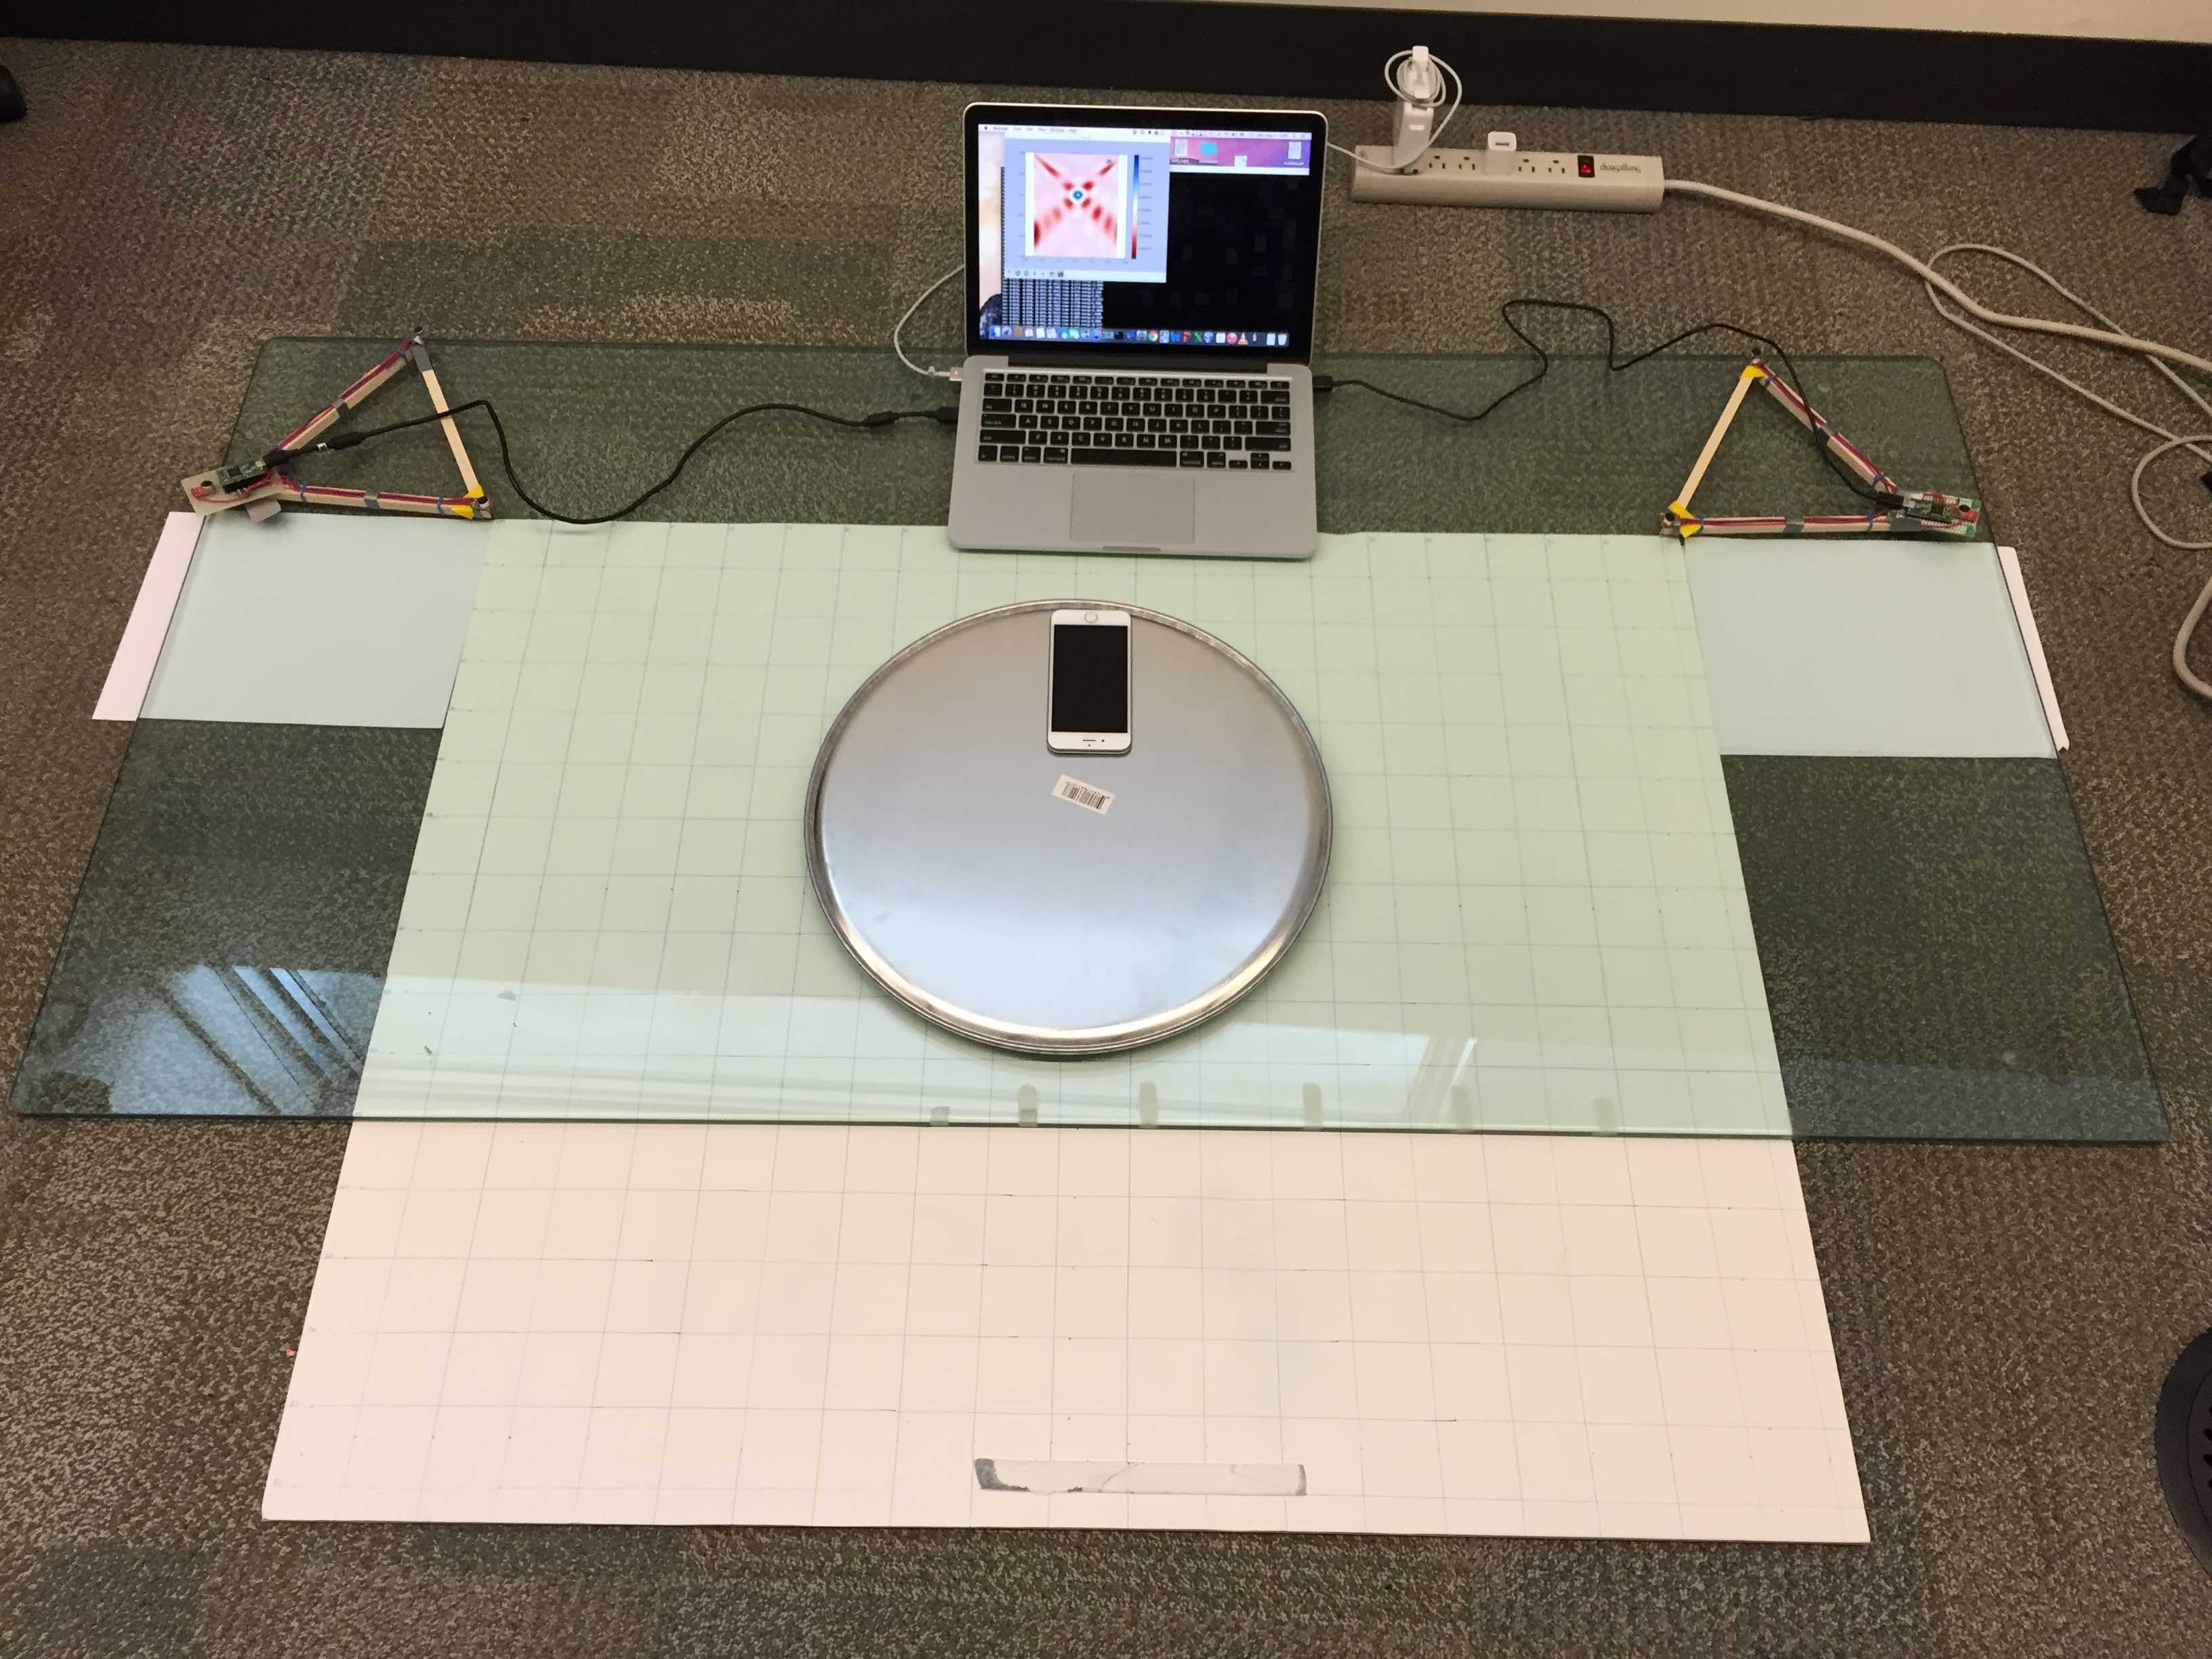
\includegraphics[width=\textwidth]{setup_rotating_disk.JPG}
  \end{subfigure}
  \caption{Setup for movement tracking evaluation}
  \label{fig:setup_circle}
\end{figure}


\begin{figure*}[]
\centering
  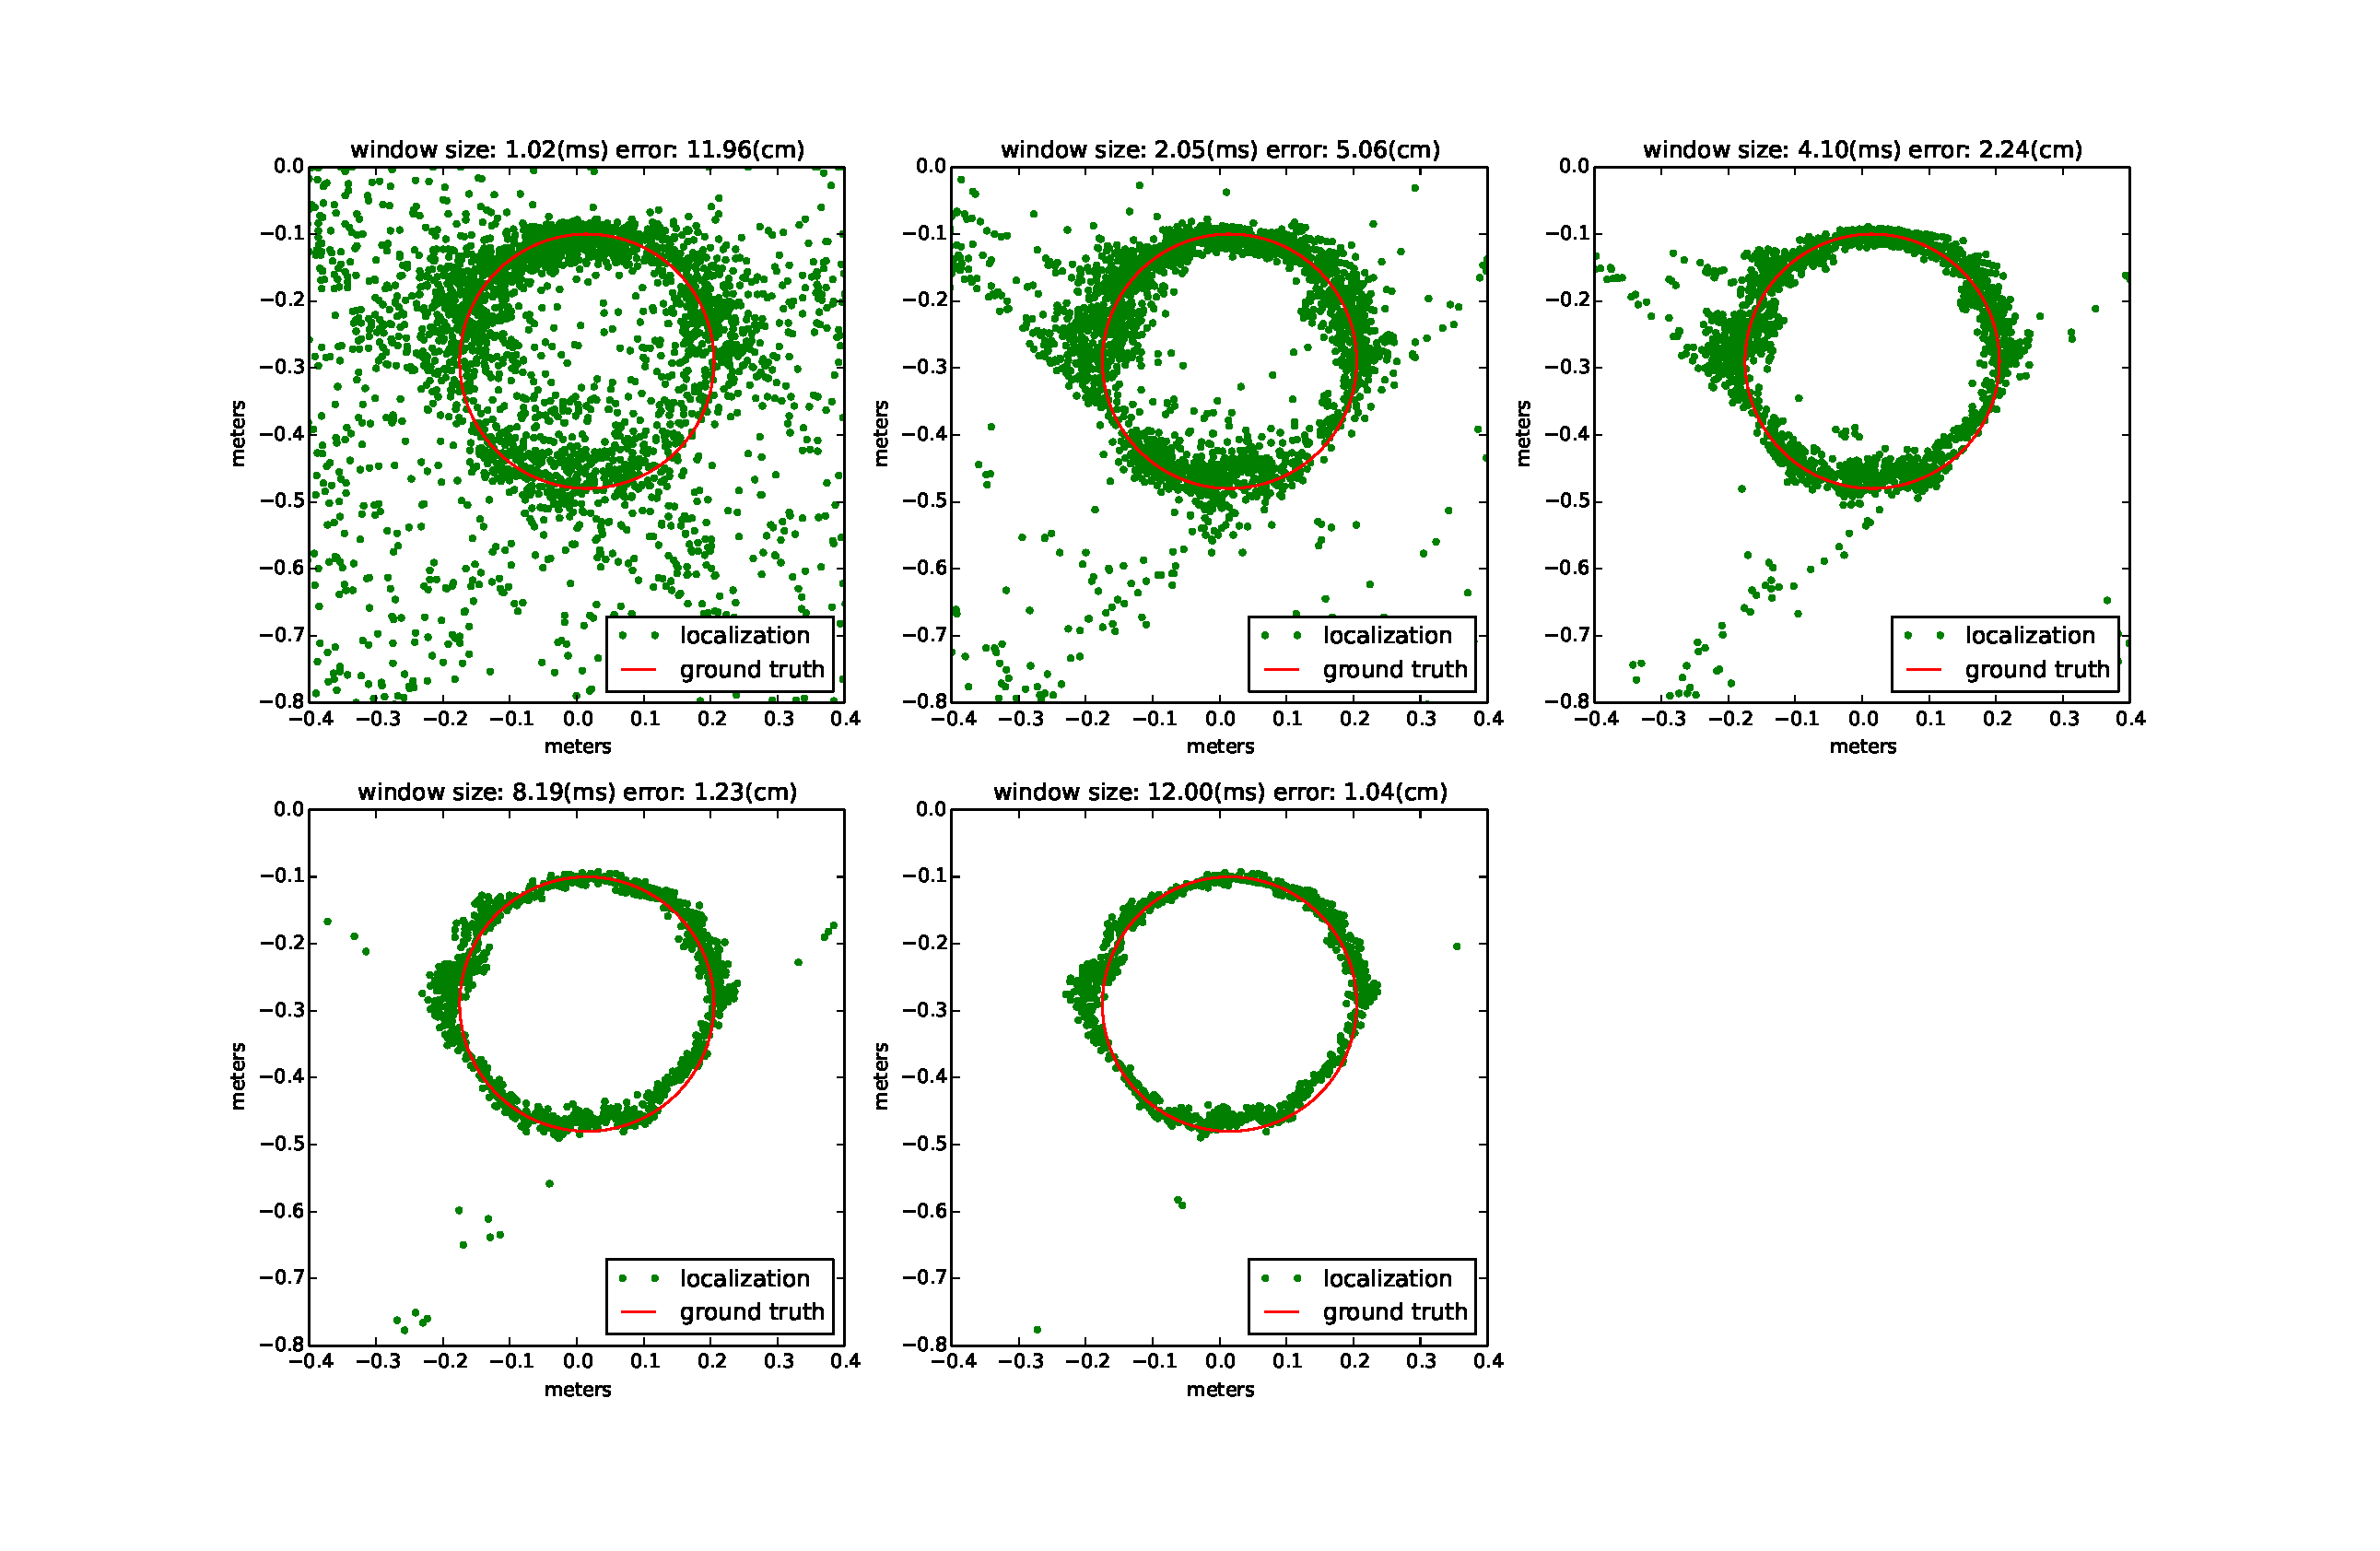
\includegraphics[width=\textwidth]{trace_window_size_movement.eps}
\caption{Localization quality versus window size}\label{fig:wn}
\label{fig:trace_win_circle}
\end{figure*}

\begin{figure}[]
\centering
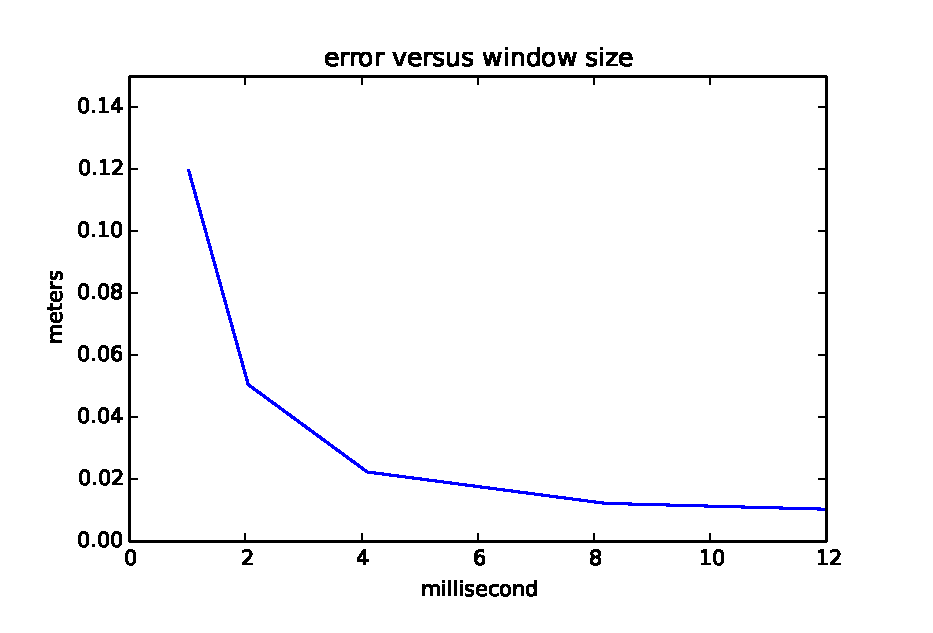
\includegraphics[width=1.0\textwidth]{error_window_size_movement.eps}
\caption{Localization error versus window size}
\label{fig:err_win_circle}
\end{figure}


\subsection{Movement tracking}

Fig~\ref{fig:wn} gives an intuitive representation of how accuracy changes with window size. When window size is small ($1.02$ millisecond), the audio does not contain enough information to reliably estimate TDOA, which results in noisy localization. As window size increases, localization converges to the shape of the ground truth circle. Fig~\ref{fig:err_win_circle} shows how the error changes with window size. The general trend is similar to that in point localization case. Error decreases as the window size increases and plateaus after it exceeds around $10$ milliseconds.

\begin{figure*}[]
\centering
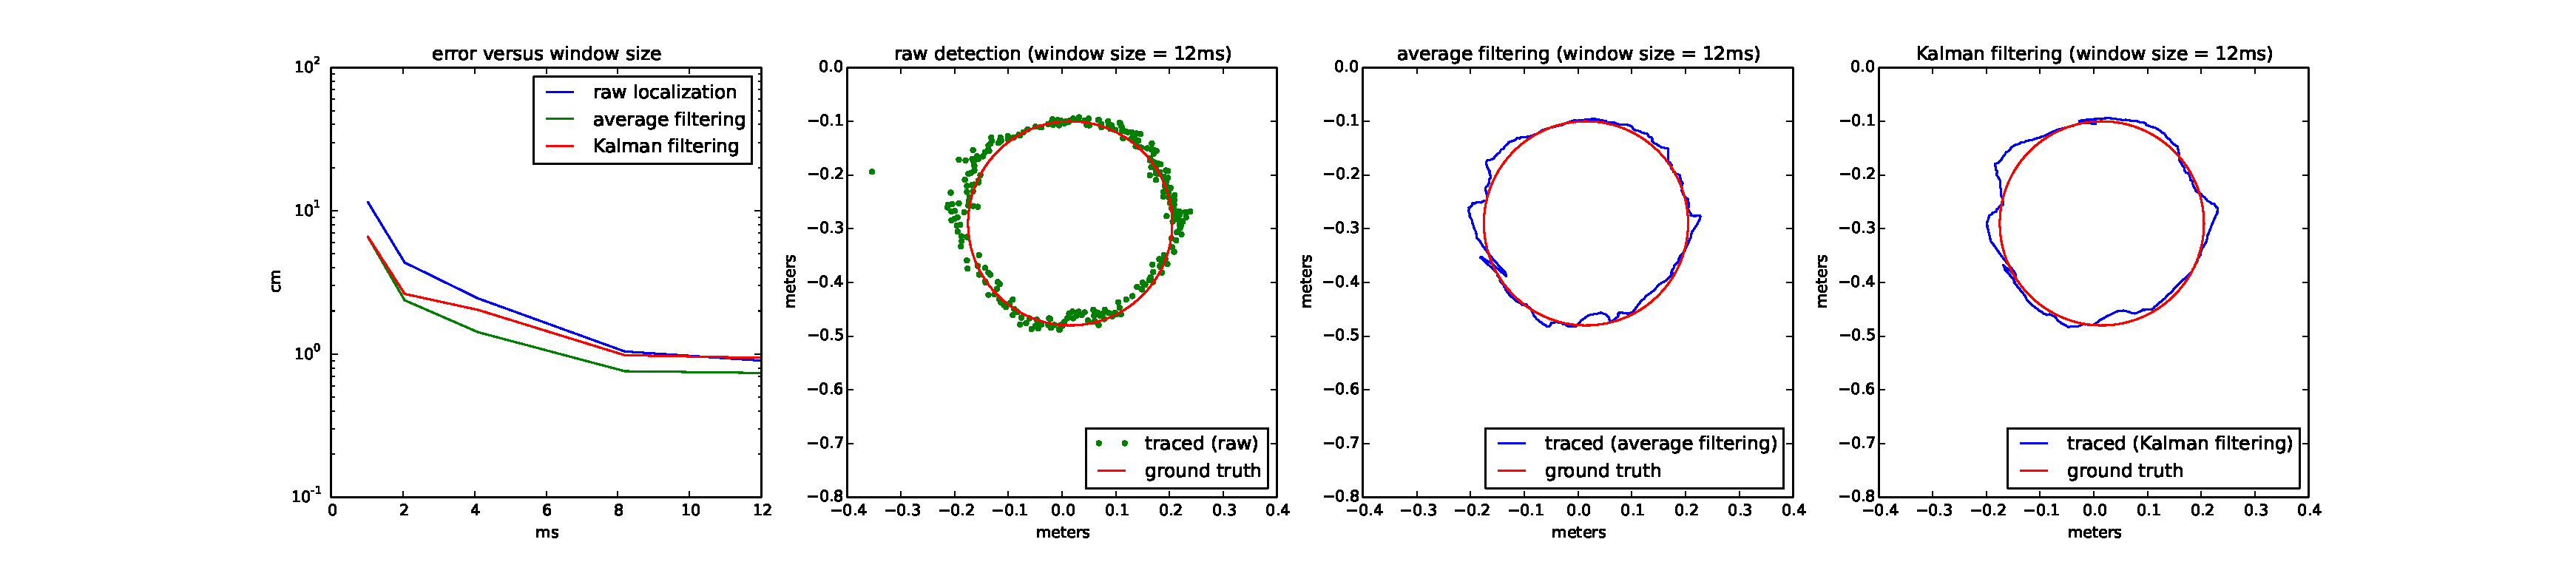
\includegraphics[width=1.0\textwidth]{trace_output_circle_wnn.eps}
\caption{white noise ($10$ cm per second)}
\label{fig:circle_wnn}
\end{figure*}

\begin{figure*}[]
\centering
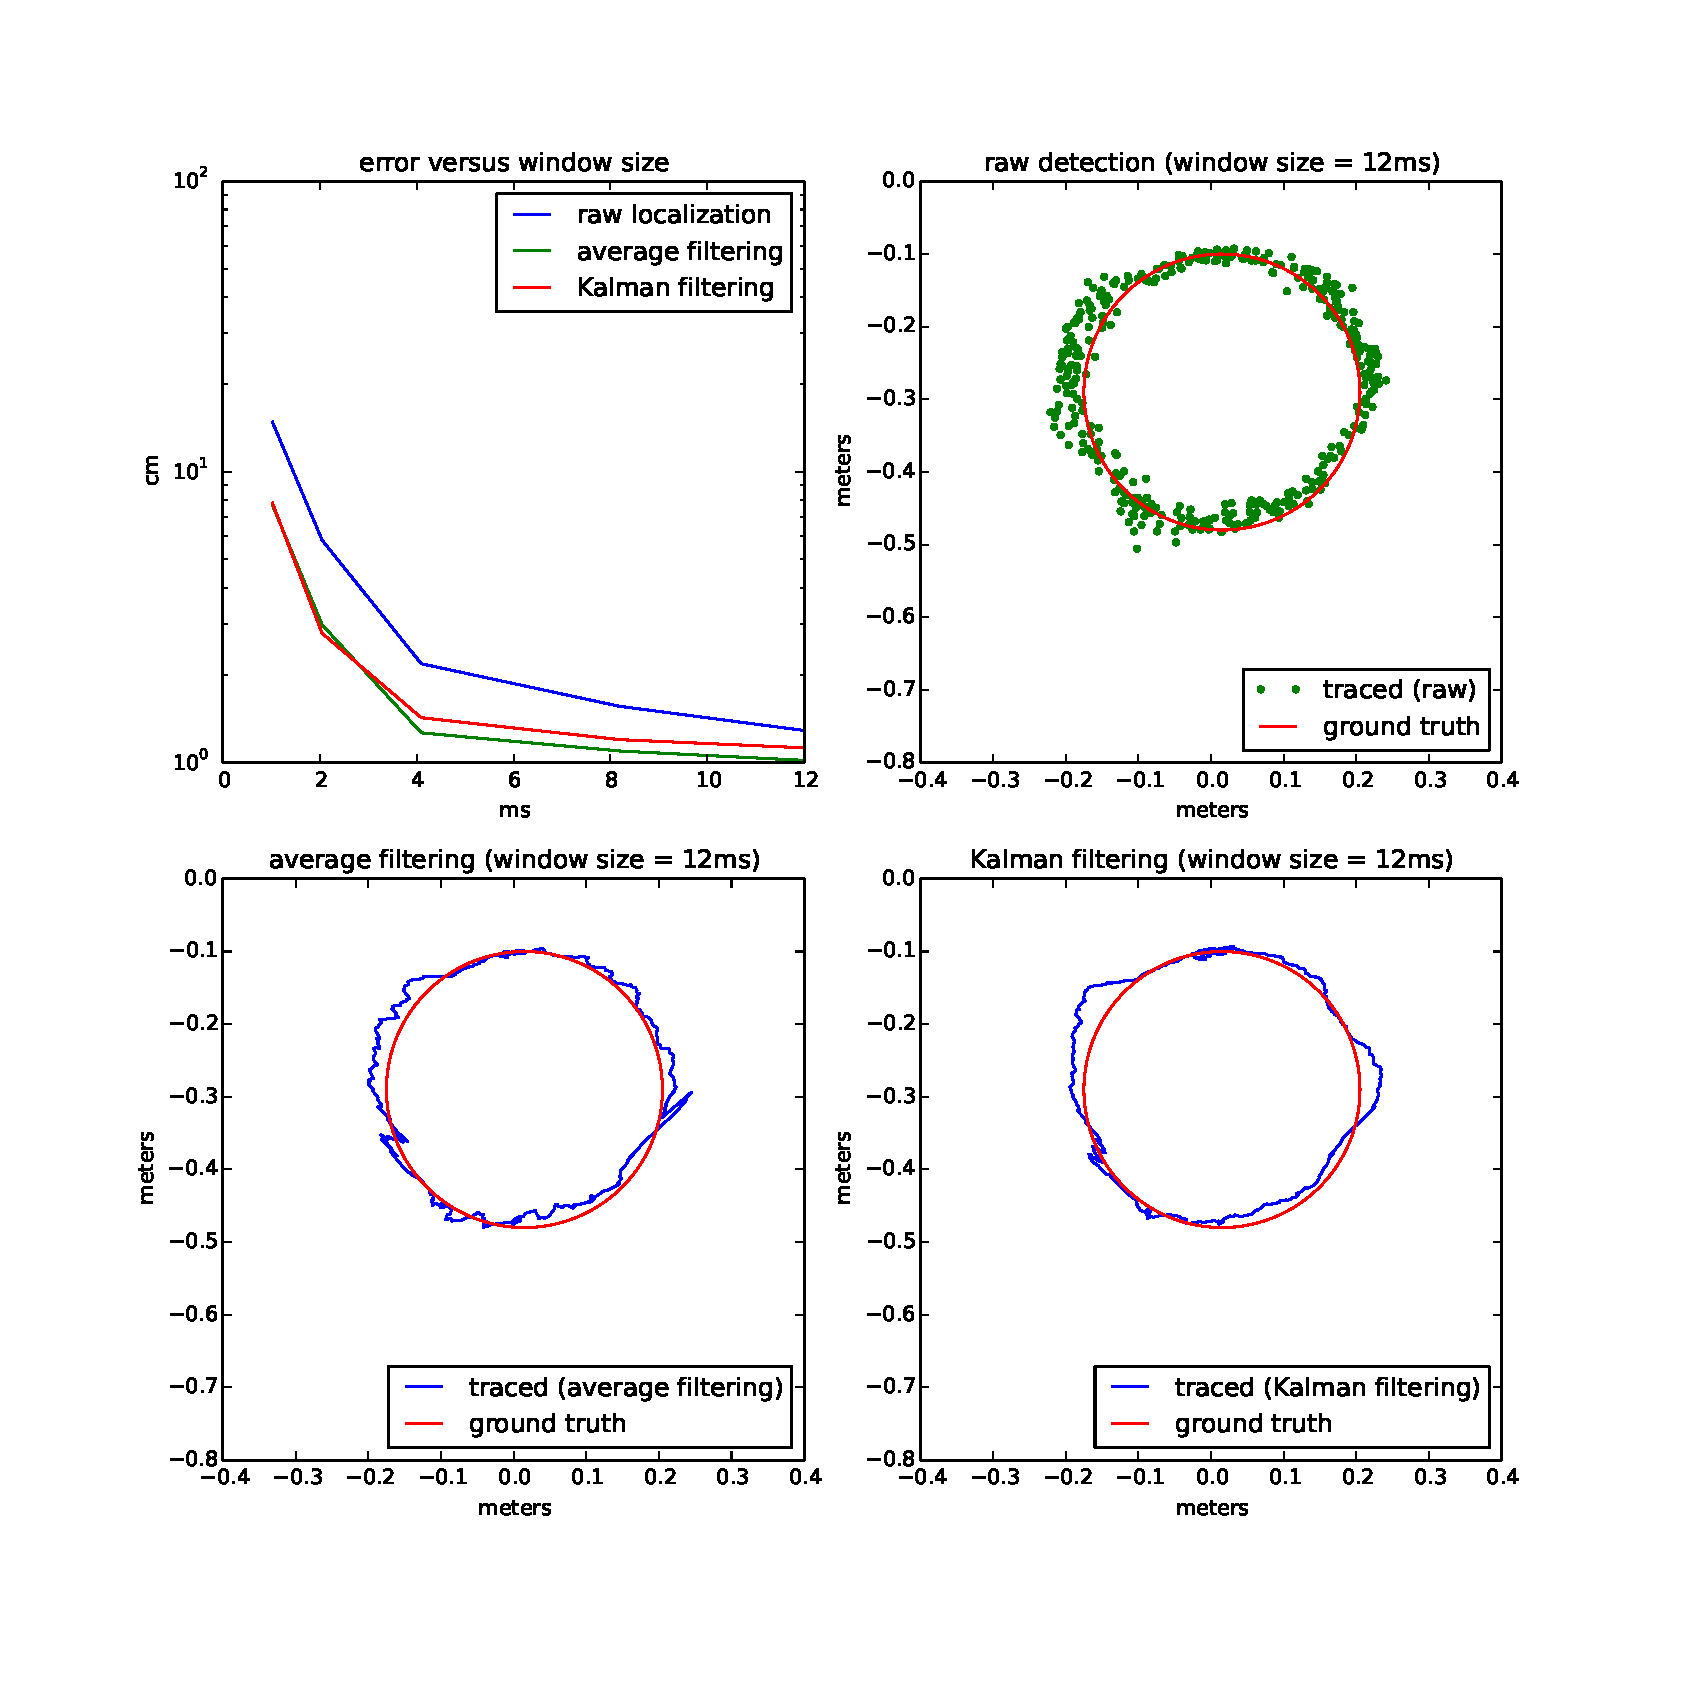
\includegraphics[width=1.0\textwidth]{trace_output_circle_man.eps}
\caption{music A ($10$ cm per second)}
\label{fig:circle_musican}
\end{figure*}

\begin{figure*}[]
\centering
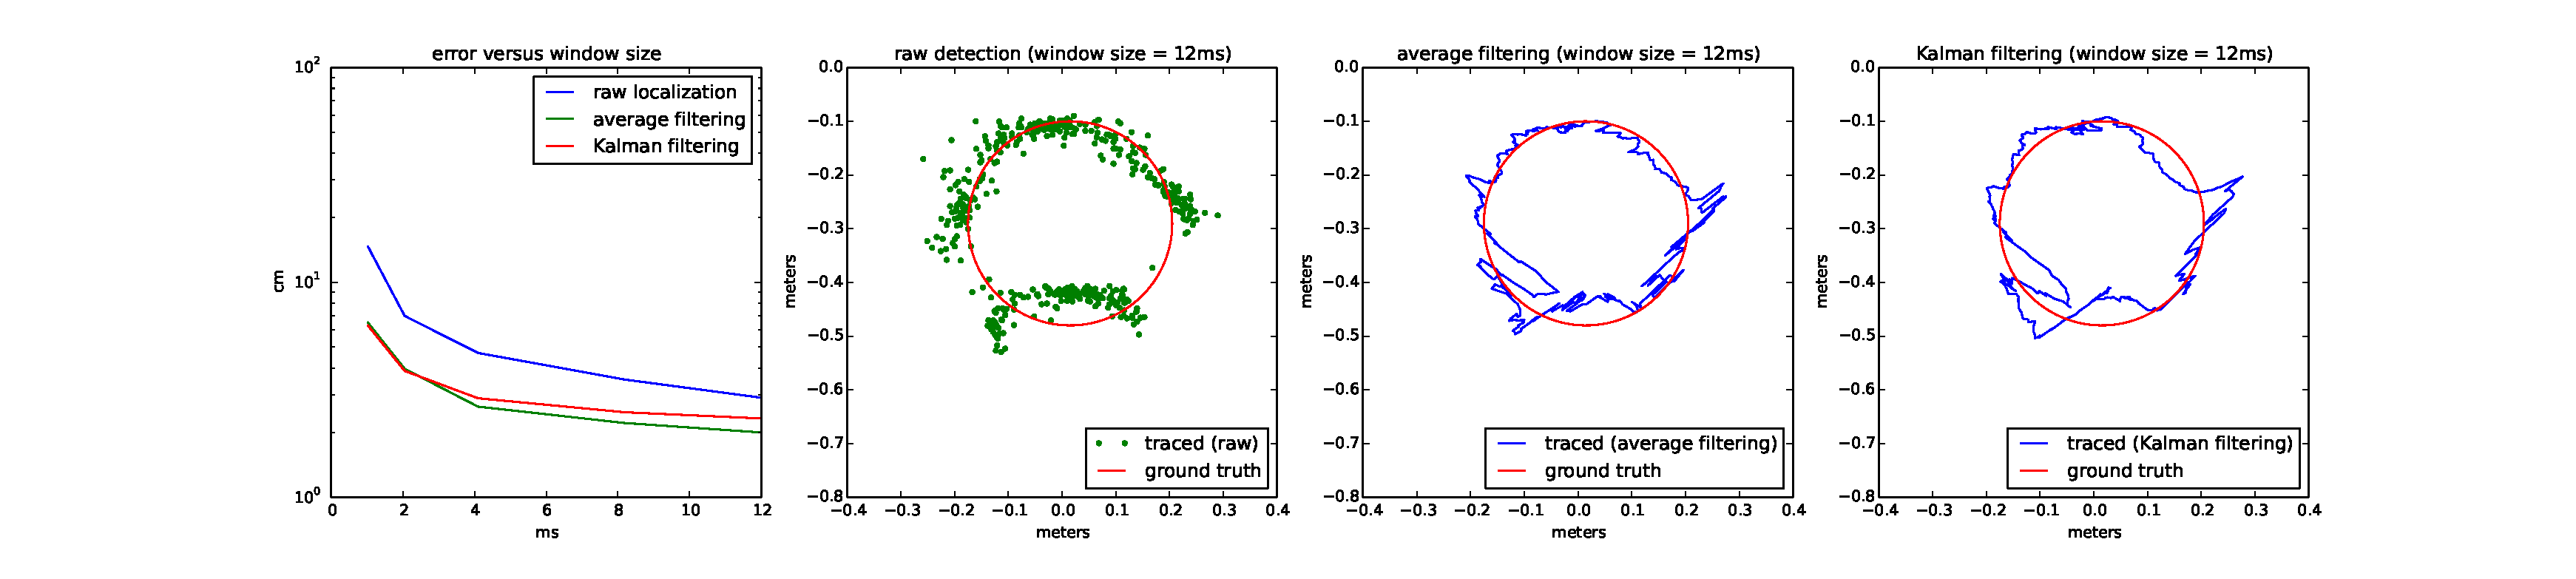
\includegraphics[width=1.0\textwidth]{trace_output_circle_mbn.eps}
\caption{music B ($10$ cm per second)}
\label{fig:circle_musicbn}
\end{figure*}

\begin{figure*}[]
\centering
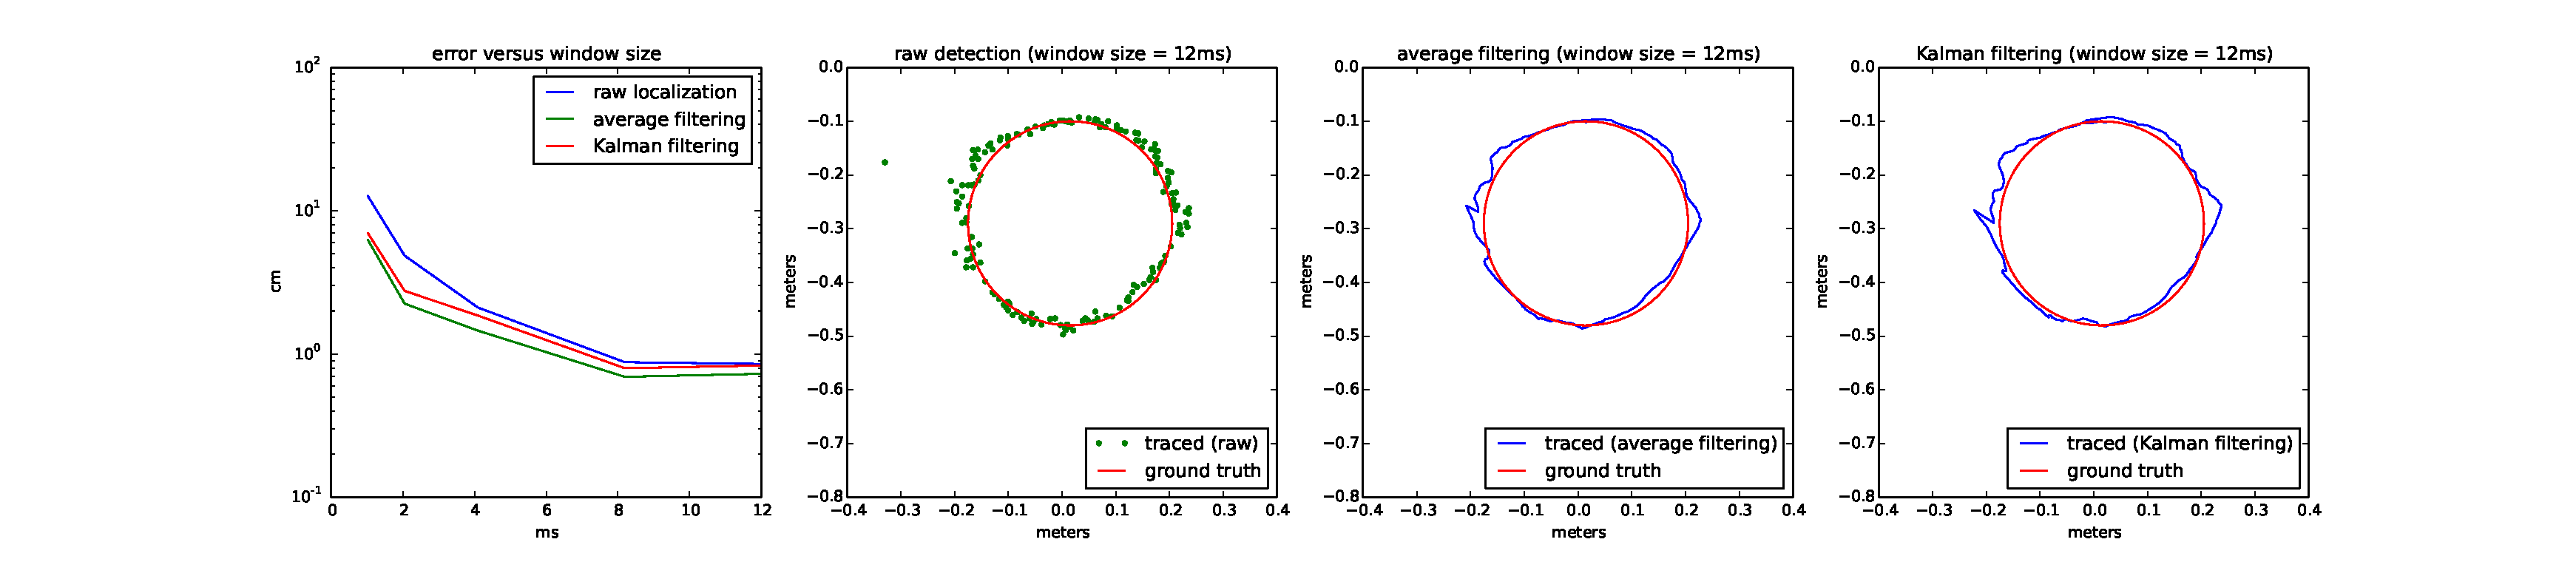
\includegraphics[width=1.0\textwidth]{trace_output_circle_wnf.eps}
\caption{white noise ($20$ cm per second)}
\label{fig:circle_wnf}
\end{figure*}

\begin{figure*}[]
\centering
  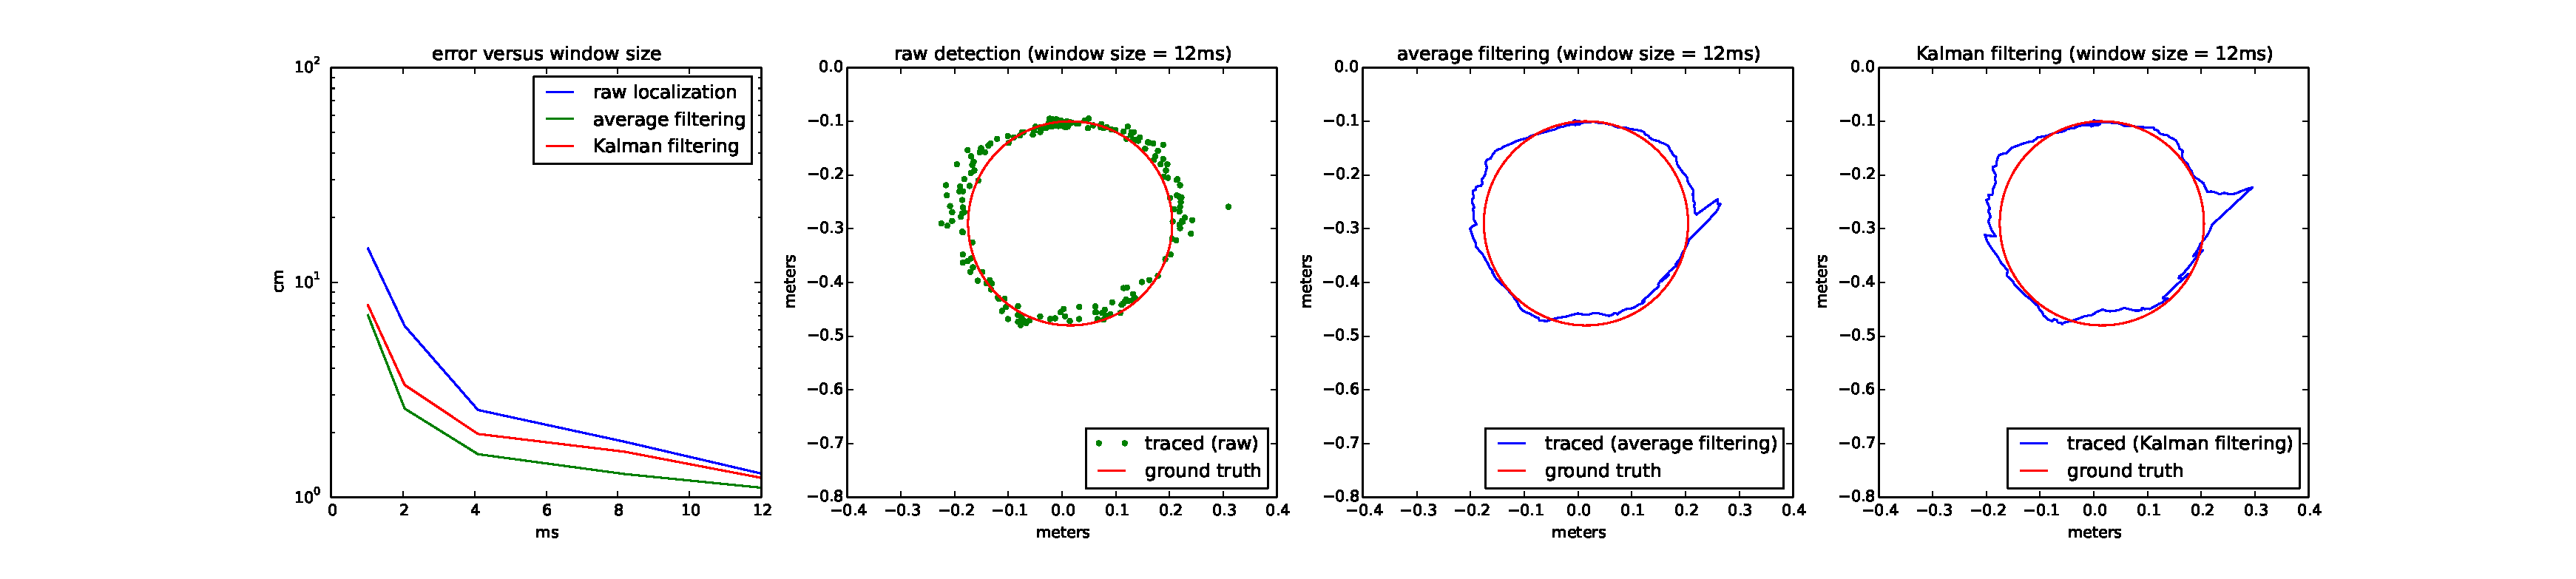
\includegraphics[width=1.0\textwidth]{trace_output_circle_maf.eps}
  \caption{music A ($20$ cm per second)}
  \label{fig:circle_musicaf}
\end{figure*}

\begin{figure*}[]
\centering
  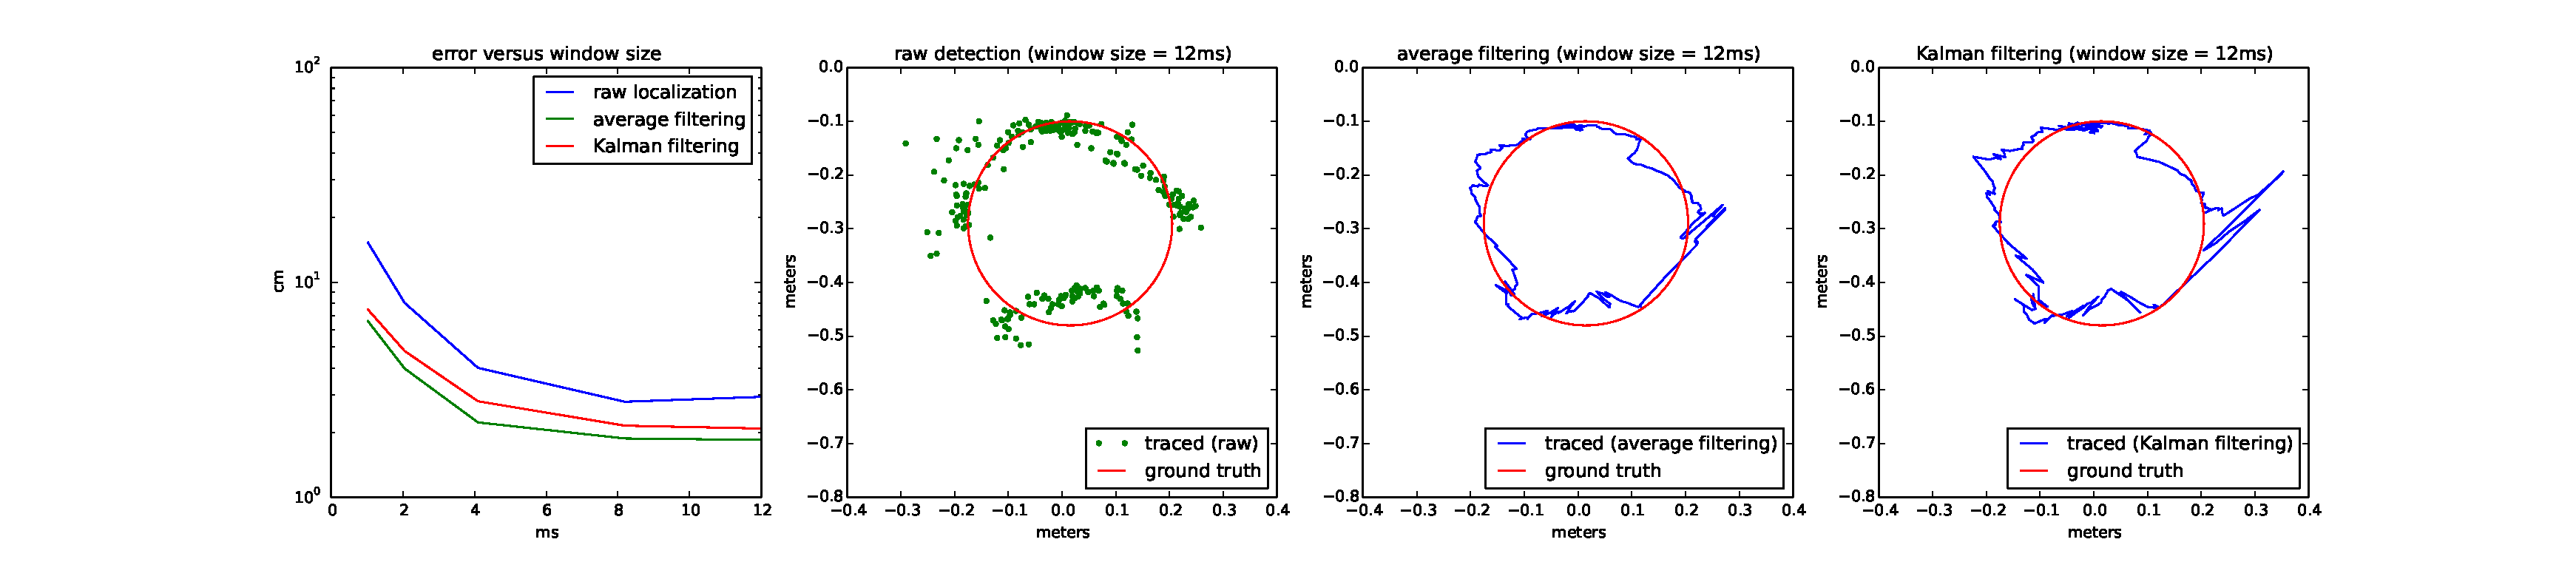
\includegraphics[width=1.0\textwidth]{trace_output_circle_mbf.eps}
  \caption{music B ($20$ cm per second)}
  \label{fig:circle_musicbf}
\end{figure*}

Fig~\ref{fig:circle_wnn} to \ref{fig:circle_musicbn} shows results for experiments at normal speed, and Fig~\ref{fig:circle_wnf} to~\ref{fig:circle_musicbf} shows results at fast speed. By comparing localization error for each audio source between normal movement speed and fast movement speed, we find that localization error does not depend on how fast the sound source is moving. For example fig~\ref{fig:circle_musican} and fig~\ref{fig:circle_musicaf} shows that localization error is $1.289$ cm at normal movement speed and $1.291$ cm at fast movement speed.

For normal speed movement tracking, localization error is $0.9$ cm for white noise, $1.29$ cm for Music A, and $2.9$ cm for Music B. Localization accuracy is the best for white noise source, and worst for Music B. This is consistent with our expectation because low amplitude regions in Music B would cause arrays to lose track of where the source is. This can also be seen from the ``blank'' regions in fig~\ref{fig:circle_musicbn}.

It also shows that raw detection has the most amount of jiggling. Kalman filter reduces the amount of jiggling from raw detection. Averaging filter has the least amount of jiggling. However, averaging filter averages detection outputs from past 0.5 seconds, which makes the filtered output lag the real movement. 
